\icode{E-MV-CA-L3-261011-002}
如图所示，一列简谐横波沿\(x\)轴传播，\(t=\) \,\qty{0.2}{s}时刻的波形如图中实线所示，\(t=\) \,\qty{0.5}{s}时刻的波形如图中虚线所示，周期\(T >\) \,\qty{5}{s}，求这列波传播的方向及传播的速度。

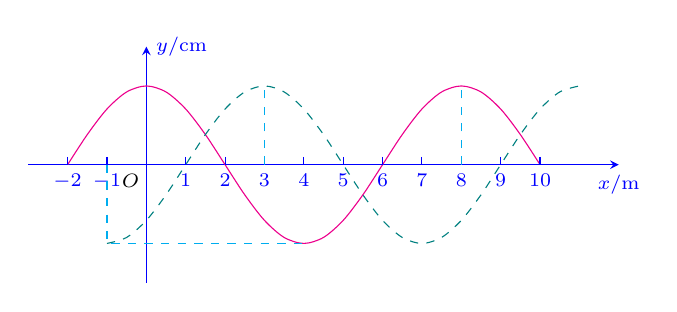
\begin{tikzpicture}[>=stealth,font=\scriptsize]
	\draw[->,blue] (0,-1.5)--(0,1.5)node[right]{\(y\)/\qty{}{cm}};
	\draw[->,blue] (-1.5,0)--(6,0)node[below]{\(x\)/\qty{}{m}};
	\draw[domain=-1:5,smooth,magenta] plot(\x,{cos(pi*\x/2 r)});
	\draw[domain=-.5:5.5,smooth,dashed,teal] plot(\x,{sin((pi*\x/2-pi/4) r)});
	\foreach \x in {-1,-.5,.5,1,...,5}
		\draw[blue] (\x,.1)--(\x,0);
	\foreach \x/\n in{-1/-2,-.5/-1,.5/1,1/2,1.5/3,2/4,2.5/5,3/6,3.5/7,4/8,4.5/9,5/10}
		\node at(\x,0)[below,blue]{\(\n\)};
	\draw[dashed,cyan] (-.5,0)--(-.5,-1)--(2,-1) (1.5,0)--(1.5,1) (4,0)--(4,1);
	\node at(-.2,-.2){\(O\)};
\end{tikzpicture}
\begin{answer}
    沿\(x\)轴正向传播，波速\qty{10}{m/s}\qquad 提示：时空转换
\end{answer}